% --------------------------------------------------------------------------------
% ---------------------------------  Preamble  -----------------------------------
% --------------------------------------------------------------------------------

\documentclass{article}

\usepackage{microtype}

\hyphenpenalty=5000 \tolerance=2000 \emergencystretch=10pt

\usepackage[defaultfam,tabular]{montserrat}
\usepackage[letterpaper, margin=0.75in]{geometry}
\usepackage{graphicx}               % to insert figures
\usepackage[table,x11names]{xcolor} % colors for e-copies
\usepackage{subcaption}             % subfigures
\usepackage{placeins}               % Float barriers
\usepackage{booktabs}
\usepackage{array}
\usepackage{caption}
\usepackage{rotating}
\usepackage{multicol}
\usepackage{multirow}
\usepackage{titlesec}
\usepackage{hyperref}               % PDF hyperreferences
\usepackage{titling}
\usepackage{tikz}
\usetikzlibrary{shapes.geometric}
\usetikzlibrary{calc}
\usepackage[T1]{fontenc}
\usepackage{ifthen}
\usepackage{fancyhdr}
\usepackage{eqparbox}
\renewcommand*\oldstylenums[1]{{\fontfamily{Montserrat-TOsF}\selectfont #1}}
\usepackage{enumitem}
\setlist[itemize]{topsep=0pt}
\setlist[enumerate]{topsep=0pt}

\makeatletter
\renewcommand{\@dotsep}{10000} 
\makeatother

\newsavebox{\savefig}

\newcommand{\Vline}[1]{\vrule width #1}
\newcommand{\Hline}[1]{\noalign{\hrule height #1}}

\setcounter{secnumdepth}{0}

\titleformat{\section}[block]
  {\normalfont\fontsize{16}{17}\fontseries{ub}\selectfont}
  {\thesection\enspace}{0pt}{\centering\MakeUppercase}[\vspace{2pt}{\titlerule[2pt]}]

\titleformat{\subsection}[block]
  {{\titlerule[1pt]}\addvspace{3pt}\bfseries\centering}
  {\thesection\enspace}{0pt}{\MakeUppercase}[\vspace{3pt}{\titlerule[1pt]}]

\titleformat{\subsubsection} [block]{\bfseries}{}{0em}{\MakeUppercase}

\renewcommand\maketitlehooka{\null\mbox{}\vfill}
\renewcommand\maketitlehookd{\vfill\null}
\title{
  \fontfamily{Montserrat-TOsF}\selectfont
  \vspace{6px}
  \fontsize{50}{60}\fontseries{ub}\selectfont\textcolor{white}{\MakeUppercase{B}}\fontsize{45}{55}\fontseries{ub}\selectfont\textcolor{white}{\MakeUppercase{attle}}\fontsize{50}{60}\fontseries{ub}\selectfont\textcolor{white}{\MakeUppercase{T}}\fontsize{45}{55}\fontseries{ub}\selectfont\textcolor{white}{\MakeUppercase{ech}}\\
  \fontsize{35}{42}\fontseries{ub}\selectfont\MakeUppercase{Outworlds Wastes}\\
  ~\\
  \href{https://ko-fi.com/bleptarts}{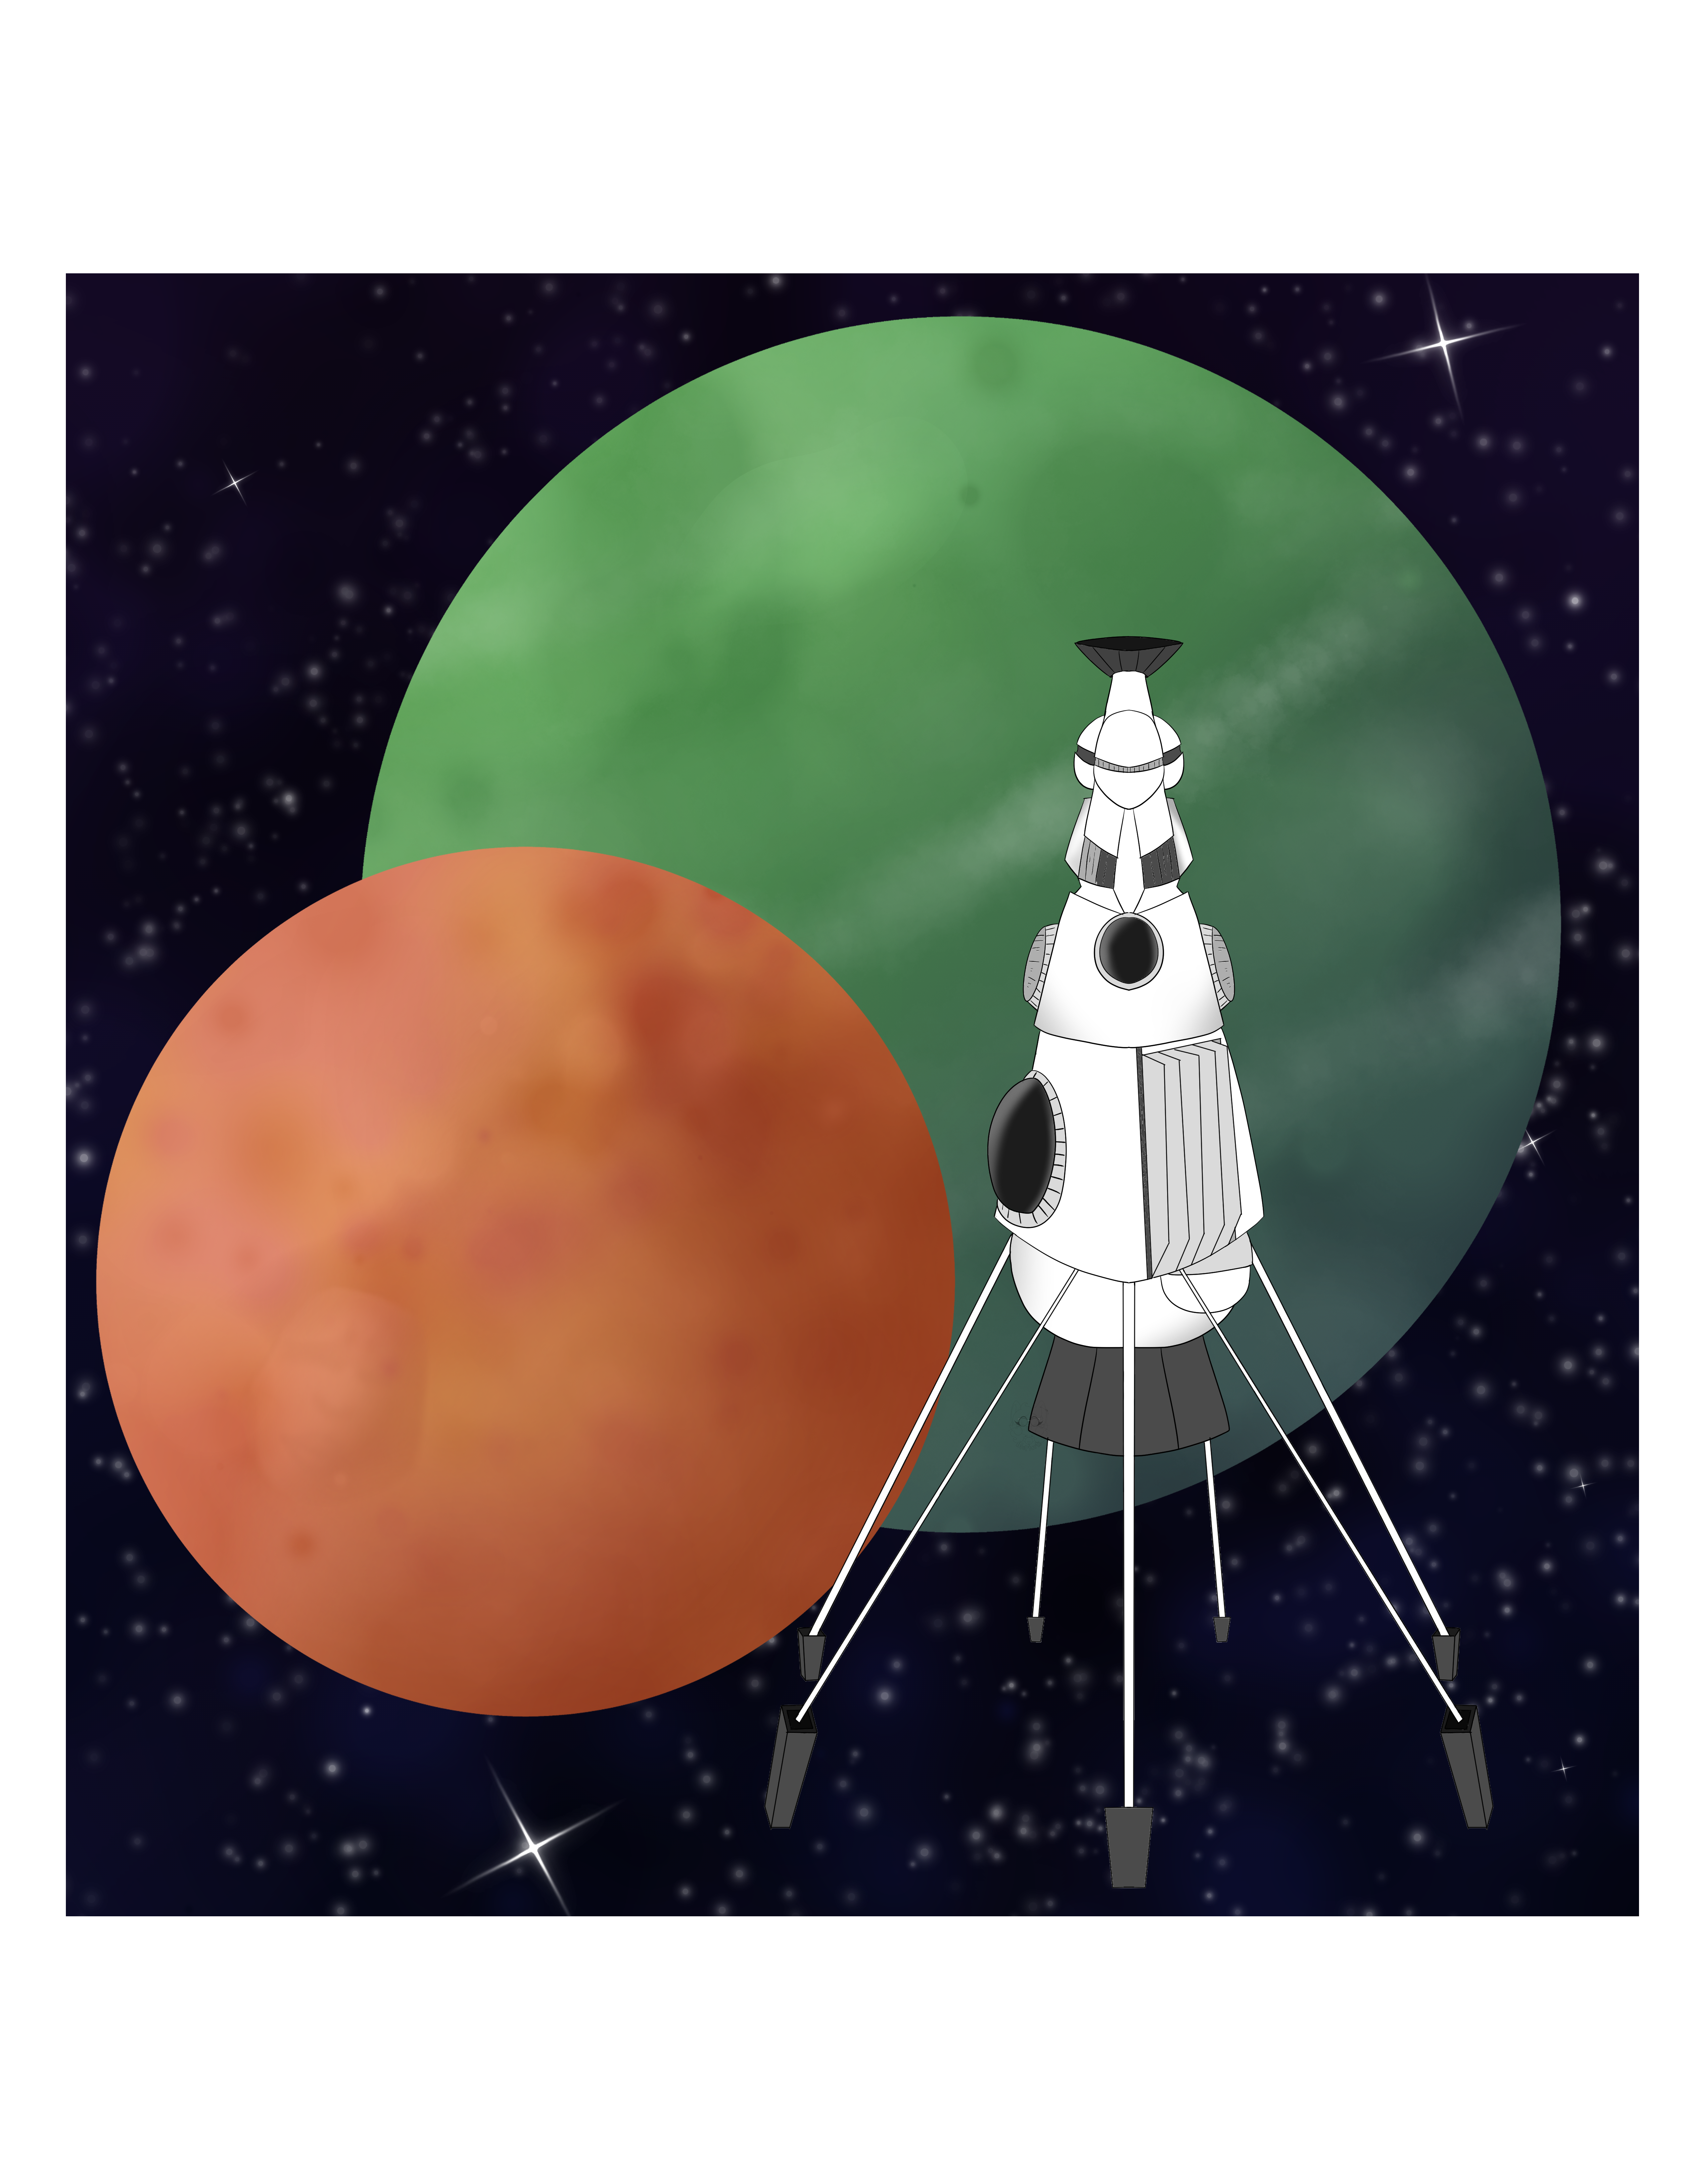
\includegraphics[alt='Outworlds Wastes logo', height=4in]{img/Outworlds-Wastes.png}}
  ~\\
  ~\\
  \LARGE\bfseries{Lightweight Narrative League Quickstart} \\
}
\author{}
\date{}

% Optional PDF information
\ifpdf
\hypersetup{
  pdftitle={Outworlds Wastes},
  pdfauthor={Jeremy L Thompson},
  pdfsubject={BattleTech},
  pdfkeywords={BattleTech}
}
\fi

\setlength\parskip{5pt plus 2pt minus 1pt}

\newcommand{\outworldsMode}{mode-pdf-quickstart}

\definecolor{background-green}{RGB}{49, 56, 49}
\definecolor{background-tan}{RGB}{204, 197, 179}
\definecolor{background-gray}{RGB}{255, 252, 247}

% --------------------------------------------------------------------------------
% ---------------------------------  Document  -----------------------------------
% --------------------------------------------------------------------------------

\begin{document}

\pagestyle{fancy}
\fancyhead{}
\renewcommand{\headrulewidth}{2pt}% default is 0pt
\fancyfoot{}
\renewcommand{\footrulewidth}{0.4pt}% default is 0pt
\fancyfoot[C]{\eqmakebox[text][r]{BattleTech} \hspace{0.1em} \eqmakebox[num][c]{\bfseries\LARGE \raisebox{-.2ex}{\thepage}} \hspace{0.1em} \eqmakebox[text][l]{Outworlds Wastes}}
\fancyfoot[R]{\footnotesize Quickstart Rules}

\clearpage

% --------------------------------------------------------------------------------
\maketitle
% --------------------------------------------------------------------------------

\AddToHookNext{shipout/background}
{\put(0,-\paperheight)
  {%
   
\begin{tikzpicture}
   \fill[use as bounding box,background-tan] (current page.north west) rectangle (\paperwidth,0);
   \fill[use as bounding box,background-green] ($ (current page.north west)+(0,-5.35) $) rectangle ++(\paperwidth,-1.7);
   \fill[use as bounding box,background-gray] ($ (current page.north west)+(0,-7.05) $) rectangle ++(\paperwidth,-1.6);
   \fill[use as bounding box,background-gray] ($ (current page.north west)+(0,-21.5) $) rectangle ++(\paperwidth,-0.9);
   \end{tikzpicture}
  }
}

\thispagestyle{empty}

\pagenumbering{roman}
\newpage
\pagenumbering{arabic}

\setlength{\headsep}{10pt}

% --------------------------------------------------------------------------------
\section{BattleTech: Outworlds Wastes Quickstart Rules}
% --------------------------------------------------------------------------------

The event format provides faster, simplified rules which are more suitable for playing multiple scenarios in a large event, such as at a convention.


% --------------------------------------------------------------------------------
\subsection{Force Maintenance and Improvements}
\label{subsec:force_maintenance}
% --------------------------------------------------------------------------------

Possible force improvements are listed below.
C-bill costs for all units are listed on the \href{http://www.masterunitlist.info}{Master Unit List}.
The C-bill cost in \href{https://megamek.org}{MegaMekLab} can be used if the \href{http://www.masterunitlist.info}{Master Unit List} does not list a cost.

\begin{itemize}

\item {\bfseries Train}: Pay 500,000 C-bills multiplied by the difference in BV skill multiplier to improve a unit's skill levels.
For example, a Gunnery 4/Piloting 5 pilot has a BV skill multiplier of 1.0 and a 3/4 pilot has a BV skill multiplier of 1.32.
Therefore, it costs 160,000 C-bills to train a 4/5 pilot to be a 3/4 pilot.
All units cannot be upgraded past 1/2.
New units cannot be upgraded past 3/4.
Old units that did not participate in the most recent scenario cannot be upgraded past 4/5.
See \emph{BattleTech: TechManual}, page 315, for the BV skill multiplier table.
A unit's skill levels can be degraded at no C-bill cost.
ProtoMechs and infantry units that cannot make anti-'Mech attacks have Piloting/Anti-'Mech 5.

\item {\bfseries Replace}: Pay 50\% of the C-bill cost, rounded up, to replace a \emph{destroyed} unit.
If the pilot or crew was killed, the replacement cost includes a 5/6 pilot.
If an entire infantry or Battle Armor unit was destroyed, the replacement cost includes 5/6 troops.
The new unit can be trained as above.
For Omni units, the replacement cost is based upon the cost of the variant on the unit roster.
See \emph{BattleTech: Total Warfare} for the definition of \emph{destroyed} for different types of units.
An abandoned unit is considered \emph{destroyed} if the commander does not control the field at the end of the scenario.

\item {\bfseries Repair}: Pay 25\% of the C-bill cost, rounded up, to repair all internal damage and critical components for a unit that has not been \emph{destroyed}.
If the pilot or crew was killed, the repair cost includes a 5/6 pilot.
Armor is repaired for free.
For Omni units, the repair cost is based upon the fielded variant.

\item {\bfseries Recruit}: Pay 50\% of the C-bill cost, rounded up, recruit new troops to replace troops in an infantry or Battle Armor unit that was not \emph{destroyed}.
For example, to recruit 1 troop in a squad of 4 IS Standard Battle Armor with Lasers, pay 50\% of the cost of 1 troop, which is 293,125 C-bills.
Damage to Battle Armor troops that survive a scenario is repaired for free.
Use the \emph{Repair} rules for Battle Armor and infantry units damaged in an Alpha Strike scenario.

\item {\bfseries Refit}: Pay the difference in C-bill cost to refit a unit to a different variant.
A Phoenix Hawk PXH-2 costs 4,348,840 C-bills and a Phoenix Hawk PXH-1K costs 3,628,553.
A commander may pay 720,287 C-bills to convert a PHX-2 into a PHX-1K or to convert a PHX-1K into a PHX-2.
Note that it still costs C-bills to refit when the new variant is cheaper.
Refitting has a minimum cost of 250,000 C-bills or 10\% of the original C-bill cost of the unit, whichever is less.

\item {\bfseries Omni Refit}: OmniMechs and Battle Armor with modular weapon mounts can be temporarily configured as a cheaper variant at no cost.
For example, the Carrion Crow C costs 10,336,492 C-bills.
The Carrion Crow A costs 9,704,829 C-bills, so a Carrion Crow C can be temporarily configured as a Carrion Crow A for a scenario.
A Carrion Crow B costs 15,617,992 C-bills, so a Carrion Crow C cannot be configured as a Carrion Crow B.
If the Carrion Crow C is refit to a Carrion Crow B, then the unit can be configured as a Carrion Crow A, B, or C for any scenario.

\item {\bfseries Purchase}: Pay the C-bill cost to get a new unit.
Commanders must purchase units from their \href{http://www.masterunitlist.info}{Master Unit List} faction and era list.
The new unit has a pilot/crew at skill 4/5 and can be trained.

\item {\bfseries Salvage}: Pay 50\% the C-bill cost, rounded up, to salvage enemy units that that were destroyed in a scenario.
A War Crow Prime costs 22,057,358 C-bills, and a salvaged War Crow Prime costs 11,028,679 C-bills.
The new unit starts at skill 4/5 and can be trained.
Alternatively, commanders can earn 25\% of the C-bill cost by selling a salvaged unit.
A salvaged War Crow Prime could be sold to earn 5,514,340 C-bills instead of paying 11,028,679 C-bills to repair it.

\item {\bfseries Sell}: Commanders can sell units for 50\% of the C-bill cost or destroyed units for 25\% of the C-bill cost, rounded up.
A Locust LCT-1E costs 1,574,200 C-bills and can be sold for 787,100 C-bills.
If the Locust LCT-1E was destroyed, then selling it would only yield 393,550 C-bills.

\end{itemize}



\newpage

% --------------------------------------------------------------------------------
\tableofcontents
% --------------------------------------------------------------------------------

\newpage

% --------------------------------------------------------------------------------
\section{Background}
% --------------------------------------------------------------------------------

The event format provides faster, simplified rules which are more suitable for playing multiple scenarios in a large event, such as at a convention.


% --------------------------------------------------------------------------------
\subsection{Force Maintenance and Improvements}
\label{subsec:force_maintenance}
% --------------------------------------------------------------------------------

Possible force improvements are listed below.
C-bill costs for all units are listed on the \href{http://www.masterunitlist.info}{Master Unit List}.
The C-bill cost in \href{https://megamek.org}{MegaMekLab} can be used if the \href{http://www.masterunitlist.info}{Master Unit List} does not list a cost.

\begin{itemize}

\item {\bfseries Train}: Pay 500,000 C-bills multiplied by the difference in BV skill multiplier to improve a unit's skill levels.
For example, a Gunnery 4/Piloting 5 pilot has a BV skill multiplier of 1.0 and a 3/4 pilot has a BV skill multiplier of 1.32.
Therefore, it costs 160,000 C-bills to train a 4/5 pilot to be a 3/4 pilot.
All units cannot be upgraded past 1/2.
New units cannot be upgraded past 3/4.
Old units that did not participate in the most recent scenario cannot be upgraded past 4/5.
See \emph{BattleTech: TechManual}, page 315, for the BV skill multiplier table.
A unit's skill levels can be degraded at no C-bill cost.
ProtoMechs and infantry units that cannot make anti-'Mech attacks have Piloting/Anti-'Mech 5.

\item {\bfseries Replace}: Pay 50\% of the C-bill cost, rounded up, to replace a \emph{destroyed} unit.
If the pilot or crew was killed, the replacement cost includes a 5/6 pilot.
If an entire infantry or Battle Armor unit was destroyed, the replacement cost includes 5/6 troops.
The new unit can be trained as above.
For Omni units, the replacement cost is based upon the cost of the variant on the unit roster.
See \emph{BattleTech: Total Warfare} for the definition of \emph{destroyed} for different types of units.
An abandoned unit is considered \emph{destroyed} if the commander does not control the field at the end of the scenario.

\item {\bfseries Repair}: Pay 25\% of the C-bill cost, rounded up, to repair all internal damage and critical components for a unit that has not been \emph{destroyed}.
If the pilot or crew was killed, the repair cost includes a 5/6 pilot.
Armor is repaired for free.
For Omni units, the repair cost is based upon the fielded variant.

\item {\bfseries Recruit}: Pay 50\% of the C-bill cost, rounded up, recruit new troops to replace troops in an infantry or Battle Armor unit that was not \emph{destroyed}.
For example, to recruit 1 troop in a squad of 4 IS Standard Battle Armor with Lasers, pay 50\% of the cost of 1 troop, which is 293,125 C-bills.
Damage to Battle Armor troops that survive a scenario is repaired for free.
Use the \emph{Repair} rules for Battle Armor and infantry units damaged in an Alpha Strike scenario.

\item {\bfseries Refit}: Pay the difference in C-bill cost to refit a unit to a different variant.
A Phoenix Hawk PXH-2 costs 4,348,840 C-bills and a Phoenix Hawk PXH-1K costs 3,628,553.
A commander may pay 720,287 C-bills to convert a PHX-2 into a PHX-1K or to convert a PHX-1K into a PHX-2.
Note that it still costs C-bills to refit when the new variant is cheaper.
Refitting has a minimum cost of 250,000 C-bills or 10\% of the original C-bill cost of the unit, whichever is less.

\item {\bfseries Omni Refit}: OmniMechs and Battle Armor with modular weapon mounts can be temporarily configured as a cheaper variant at no cost.
For example, the Carrion Crow C costs 10,336,492 C-bills.
The Carrion Crow A costs 9,704,829 C-bills, so a Carrion Crow C can be temporarily configured as a Carrion Crow A for a scenario.
A Carrion Crow B costs 15,617,992 C-bills, so a Carrion Crow C cannot be configured as a Carrion Crow B.
If the Carrion Crow C is refit to a Carrion Crow B, then the unit can be configured as a Carrion Crow A, B, or C for any scenario.

\item {\bfseries Purchase}: Pay the C-bill cost to get a new unit.
Commanders must purchase units from their \href{http://www.masterunitlist.info}{Master Unit List} faction and era list.
The new unit has a pilot/crew at skill 4/5 and can be trained.

\item {\bfseries Salvage}: Pay 50\% the C-bill cost, rounded up, to salvage enemy units that that were destroyed in a scenario.
A War Crow Prime costs 22,057,358 C-bills, and a salvaged War Crow Prime costs 11,028,679 C-bills.
The new unit starts at skill 4/5 and can be trained.
Alternatively, commanders can earn 25\% of the C-bill cost by selling a salvaged unit.
A salvaged War Crow Prime could be sold to earn 5,514,340 C-bills instead of paying 11,028,679 C-bills to repair it.

\item {\bfseries Sell}: Commanders can sell units for 50\% of the C-bill cost or destroyed units for 25\% of the C-bill cost, rounded up.
A Locust LCT-1E costs 1,574,200 C-bills and can be sold for 787,100 C-bills.
If the Locust LCT-1E was destroyed, then selling it would only yield 393,550 C-bills.

\end{itemize}



\newpage

% --------------------------------------------------------------------------------
\section{Force Construction}
% --------------------------------------------------------------------------------

The event format provides faster, simplified rules which are more suitable for playing multiple scenarios in a large event, such as at a convention.


% --------------------------------------------------------------------------------
\subsection{Force Maintenance and Improvements}
\label{subsec:force_maintenance}
% --------------------------------------------------------------------------------

Possible force improvements are listed below.
C-bill costs for all units are listed on the \href{http://www.masterunitlist.info}{Master Unit List}.
The C-bill cost in \href{https://megamek.org}{MegaMekLab} can be used if the \href{http://www.masterunitlist.info}{Master Unit List} does not list a cost.

\begin{itemize}

\item {\bfseries Train}: Pay 500,000 C-bills multiplied by the difference in BV skill multiplier to improve a unit's skill levels.
For example, a Gunnery 4/Piloting 5 pilot has a BV skill multiplier of 1.0 and a 3/4 pilot has a BV skill multiplier of 1.32.
Therefore, it costs 160,000 C-bills to train a 4/5 pilot to be a 3/4 pilot.
All units cannot be upgraded past 1/2.
New units cannot be upgraded past 3/4.
Old units that did not participate in the most recent scenario cannot be upgraded past 4/5.
See \emph{BattleTech: TechManual}, page 315, for the BV skill multiplier table.
A unit's skill levels can be degraded at no C-bill cost.
ProtoMechs and infantry units that cannot make anti-'Mech attacks have Piloting/Anti-'Mech 5.

\item {\bfseries Replace}: Pay 50\% of the C-bill cost, rounded up, to replace a \emph{destroyed} unit.
If the pilot or crew was killed, the replacement cost includes a 5/6 pilot.
If an entire infantry or Battle Armor unit was destroyed, the replacement cost includes 5/6 troops.
The new unit can be trained as above.
For Omni units, the replacement cost is based upon the cost of the variant on the unit roster.
See \emph{BattleTech: Total Warfare} for the definition of \emph{destroyed} for different types of units.
An abandoned unit is considered \emph{destroyed} if the commander does not control the field at the end of the scenario.

\item {\bfseries Repair}: Pay 25\% of the C-bill cost, rounded up, to repair all internal damage and critical components for a unit that has not been \emph{destroyed}.
If the pilot or crew was killed, the repair cost includes a 5/6 pilot.
Armor is repaired for free.
For Omni units, the repair cost is based upon the fielded variant.

\item {\bfseries Recruit}: Pay 50\% of the C-bill cost, rounded up, recruit new troops to replace troops in an infantry or Battle Armor unit that was not \emph{destroyed}.
For example, to recruit 1 troop in a squad of 4 IS Standard Battle Armor with Lasers, pay 50\% of the cost of 1 troop, which is 293,125 C-bills.
Damage to Battle Armor troops that survive a scenario is repaired for free.
Use the \emph{Repair} rules for Battle Armor and infantry units damaged in an Alpha Strike scenario.

\item {\bfseries Refit}: Pay the difference in C-bill cost to refit a unit to a different variant.
A Phoenix Hawk PXH-2 costs 4,348,840 C-bills and a Phoenix Hawk PXH-1K costs 3,628,553.
A commander may pay 720,287 C-bills to convert a PHX-2 into a PHX-1K or to convert a PHX-1K into a PHX-2.
Note that it still costs C-bills to refit when the new variant is cheaper.
Refitting has a minimum cost of 250,000 C-bills or 10\% of the original C-bill cost of the unit, whichever is less.

\item {\bfseries Omni Refit}: OmniMechs and Battle Armor with modular weapon mounts can be temporarily configured as a cheaper variant at no cost.
For example, the Carrion Crow C costs 10,336,492 C-bills.
The Carrion Crow A costs 9,704,829 C-bills, so a Carrion Crow C can be temporarily configured as a Carrion Crow A for a scenario.
A Carrion Crow B costs 15,617,992 C-bills, so a Carrion Crow C cannot be configured as a Carrion Crow B.
If the Carrion Crow C is refit to a Carrion Crow B, then the unit can be configured as a Carrion Crow A, B, or C for any scenario.

\item {\bfseries Purchase}: Pay the C-bill cost to get a new unit.
Commanders must purchase units from their \href{http://www.masterunitlist.info}{Master Unit List} faction and era list.
The new unit has a pilot/crew at skill 4/5 and can be trained.

\item {\bfseries Salvage}: Pay 50\% the C-bill cost, rounded up, to salvage enemy units that that were destroyed in a scenario.
A War Crow Prime costs 22,057,358 C-bills, and a salvaged War Crow Prime costs 11,028,679 C-bills.
The new unit starts at skill 4/5 and can be trained.
Alternatively, commanders can earn 25\% of the C-bill cost by selling a salvaged unit.
A salvaged War Crow Prime could be sold to earn 5,514,340 C-bills instead of paying 11,028,679 C-bills to repair it.

\item {\bfseries Sell}: Commanders can sell units for 50\% of the C-bill cost or destroyed units for 25\% of the C-bill cost, rounded up.
A Locust LCT-1E costs 1,574,200 C-bills and can be sold for 787,100 C-bills.
If the Locust LCT-1E was destroyed, then selling it would only yield 393,550 C-bills.

\end{itemize}



\newpage

% --------------------------------------------------------------------------------
\section{Force Management}
% --------------------------------------------------------------------------------

The event format provides faster, simplified rules which are more suitable for playing multiple scenarios in a large event, such as at a convention.


% --------------------------------------------------------------------------------
\subsection{Force Maintenance and Improvements}
\label{subsec:force_maintenance}
% --------------------------------------------------------------------------------

Possible force improvements are listed below.
C-bill costs for all units are listed on the \href{http://www.masterunitlist.info}{Master Unit List}.
The C-bill cost in \href{https://megamek.org}{MegaMekLab} can be used if the \href{http://www.masterunitlist.info}{Master Unit List} does not list a cost.

\begin{itemize}

\item {\bfseries Train}: Pay 500,000 C-bills multiplied by the difference in BV skill multiplier to improve a unit's skill levels.
For example, a Gunnery 4/Piloting 5 pilot has a BV skill multiplier of 1.0 and a 3/4 pilot has a BV skill multiplier of 1.32.
Therefore, it costs 160,000 C-bills to train a 4/5 pilot to be a 3/4 pilot.
All units cannot be upgraded past 1/2.
New units cannot be upgraded past 3/4.
Old units that did not participate in the most recent scenario cannot be upgraded past 4/5.
See \emph{BattleTech: TechManual}, page 315, for the BV skill multiplier table.
A unit's skill levels can be degraded at no C-bill cost.
ProtoMechs and infantry units that cannot make anti-'Mech attacks have Piloting/Anti-'Mech 5.

\item {\bfseries Replace}: Pay 50\% of the C-bill cost, rounded up, to replace a \emph{destroyed} unit.
If the pilot or crew was killed, the replacement cost includes a 5/6 pilot.
If an entire infantry or Battle Armor unit was destroyed, the replacement cost includes 5/6 troops.
The new unit can be trained as above.
For Omni units, the replacement cost is based upon the cost of the variant on the unit roster.
See \emph{BattleTech: Total Warfare} for the definition of \emph{destroyed} for different types of units.
An abandoned unit is considered \emph{destroyed} if the commander does not control the field at the end of the scenario.

\item {\bfseries Repair}: Pay 25\% of the C-bill cost, rounded up, to repair all internal damage and critical components for a unit that has not been \emph{destroyed}.
If the pilot or crew was killed, the repair cost includes a 5/6 pilot.
Armor is repaired for free.
For Omni units, the repair cost is based upon the fielded variant.

\item {\bfseries Recruit}: Pay 50\% of the C-bill cost, rounded up, recruit new troops to replace troops in an infantry or Battle Armor unit that was not \emph{destroyed}.
For example, to recruit 1 troop in a squad of 4 IS Standard Battle Armor with Lasers, pay 50\% of the cost of 1 troop, which is 293,125 C-bills.
Damage to Battle Armor troops that survive a scenario is repaired for free.
Use the \emph{Repair} rules for Battle Armor and infantry units damaged in an Alpha Strike scenario.

\item {\bfseries Refit}: Pay the difference in C-bill cost to refit a unit to a different variant.
A Phoenix Hawk PXH-2 costs 4,348,840 C-bills and a Phoenix Hawk PXH-1K costs 3,628,553.
A commander may pay 720,287 C-bills to convert a PHX-2 into a PHX-1K or to convert a PHX-1K into a PHX-2.
Note that it still costs C-bills to refit when the new variant is cheaper.
Refitting has a minimum cost of 250,000 C-bills or 10\% of the original C-bill cost of the unit, whichever is less.

\item {\bfseries Omni Refit}: OmniMechs and Battle Armor with modular weapon mounts can be temporarily configured as a cheaper variant at no cost.
For example, the Carrion Crow C costs 10,336,492 C-bills.
The Carrion Crow A costs 9,704,829 C-bills, so a Carrion Crow C can be temporarily configured as a Carrion Crow A for a scenario.
A Carrion Crow B costs 15,617,992 C-bills, so a Carrion Crow C cannot be configured as a Carrion Crow B.
If the Carrion Crow C is refit to a Carrion Crow B, then the unit can be configured as a Carrion Crow A, B, or C for any scenario.

\item {\bfseries Purchase}: Pay the C-bill cost to get a new unit.
Commanders must purchase units from their \href{http://www.masterunitlist.info}{Master Unit List} faction and era list.
The new unit has a pilot/crew at skill 4/5 and can be trained.

\item {\bfseries Salvage}: Pay 50\% the C-bill cost, rounded up, to salvage enemy units that that were destroyed in a scenario.
A War Crow Prime costs 22,057,358 C-bills, and a salvaged War Crow Prime costs 11,028,679 C-bills.
The new unit starts at skill 4/5 and can be trained.
Alternatively, commanders can earn 25\% of the C-bill cost by selling a salvaged unit.
A salvaged War Crow Prime could be sold to earn 5,514,340 C-bills instead of paying 11,028,679 C-bills to repair it.

\item {\bfseries Sell}: Commanders can sell units for 50\% of the C-bill cost or destroyed units for 25\% of the C-bill cost, rounded up.
A Locust LCT-1E costs 1,574,200 C-bills and can be sold for 787,100 C-bills.
If the Locust LCT-1E was destroyed, then selling it would only yield 393,550 C-bills.

\end{itemize}



\newpage

% --------------------------------------------------------------------------------
\section{Scenarios}
% --------------------------------------------------------------------------------

The event format provides faster, simplified rules which are more suitable for playing multiple scenarios in a large event, such as at a convention.


% --------------------------------------------------------------------------------
\subsection{Force Maintenance and Improvements}
\label{subsec:force_maintenance}
% --------------------------------------------------------------------------------

Possible force improvements are listed below.
C-bill costs for all units are listed on the \href{http://www.masterunitlist.info}{Master Unit List}.
The C-bill cost in \href{https://megamek.org}{MegaMekLab} can be used if the \href{http://www.masterunitlist.info}{Master Unit List} does not list a cost.

\begin{itemize}

\item {\bfseries Train}: Pay 500,000 C-bills multiplied by the difference in BV skill multiplier to improve a unit's skill levels.
For example, a Gunnery 4/Piloting 5 pilot has a BV skill multiplier of 1.0 and a 3/4 pilot has a BV skill multiplier of 1.32.
Therefore, it costs 160,000 C-bills to train a 4/5 pilot to be a 3/4 pilot.
All units cannot be upgraded past 1/2.
New units cannot be upgraded past 3/4.
Old units that did not participate in the most recent scenario cannot be upgraded past 4/5.
See \emph{BattleTech: TechManual}, page 315, for the BV skill multiplier table.
A unit's skill levels can be degraded at no C-bill cost.
ProtoMechs and infantry units that cannot make anti-'Mech attacks have Piloting/Anti-'Mech 5.

\item {\bfseries Replace}: Pay 50\% of the C-bill cost, rounded up, to replace a \emph{destroyed} unit.
If the pilot or crew was killed, the replacement cost includes a 5/6 pilot.
If an entire infantry or Battle Armor unit was destroyed, the replacement cost includes 5/6 troops.
The new unit can be trained as above.
For Omni units, the replacement cost is based upon the cost of the variant on the unit roster.
See \emph{BattleTech: Total Warfare} for the definition of \emph{destroyed} for different types of units.
An abandoned unit is considered \emph{destroyed} if the commander does not control the field at the end of the scenario.

\item {\bfseries Repair}: Pay 25\% of the C-bill cost, rounded up, to repair all internal damage and critical components for a unit that has not been \emph{destroyed}.
If the pilot or crew was killed, the repair cost includes a 5/6 pilot.
Armor is repaired for free.
For Omni units, the repair cost is based upon the fielded variant.

\item {\bfseries Recruit}: Pay 50\% of the C-bill cost, rounded up, recruit new troops to replace troops in an infantry or Battle Armor unit that was not \emph{destroyed}.
For example, to recruit 1 troop in a squad of 4 IS Standard Battle Armor with Lasers, pay 50\% of the cost of 1 troop, which is 293,125 C-bills.
Damage to Battle Armor troops that survive a scenario is repaired for free.
Use the \emph{Repair} rules for Battle Armor and infantry units damaged in an Alpha Strike scenario.

\item {\bfseries Refit}: Pay the difference in C-bill cost to refit a unit to a different variant.
A Phoenix Hawk PXH-2 costs 4,348,840 C-bills and a Phoenix Hawk PXH-1K costs 3,628,553.
A commander may pay 720,287 C-bills to convert a PHX-2 into a PHX-1K or to convert a PHX-1K into a PHX-2.
Note that it still costs C-bills to refit when the new variant is cheaper.
Refitting has a minimum cost of 250,000 C-bills or 10\% of the original C-bill cost of the unit, whichever is less.

\item {\bfseries Omni Refit}: OmniMechs and Battle Armor with modular weapon mounts can be temporarily configured as a cheaper variant at no cost.
For example, the Carrion Crow C costs 10,336,492 C-bills.
The Carrion Crow A costs 9,704,829 C-bills, so a Carrion Crow C can be temporarily configured as a Carrion Crow A for a scenario.
A Carrion Crow B costs 15,617,992 C-bills, so a Carrion Crow C cannot be configured as a Carrion Crow B.
If the Carrion Crow C is refit to a Carrion Crow B, then the unit can be configured as a Carrion Crow A, B, or C for any scenario.

\item {\bfseries Purchase}: Pay the C-bill cost to get a new unit.
Commanders must purchase units from their \href{http://www.masterunitlist.info}{Master Unit List} faction and era list.
The new unit has a pilot/crew at skill 4/5 and can be trained.

\item {\bfseries Salvage}: Pay 50\% the C-bill cost, rounded up, to salvage enemy units that that were destroyed in a scenario.
A War Crow Prime costs 22,057,358 C-bills, and a salvaged War Crow Prime costs 11,028,679 C-bills.
The new unit starts at skill 4/5 and can be trained.
Alternatively, commanders can earn 25\% of the C-bill cost by selling a salvaged unit.
A salvaged War Crow Prime could be sold to earn 5,514,340 C-bills instead of paying 11,028,679 C-bills to repair it.

\item {\bfseries Sell}: Commanders can sell units for 50\% of the C-bill cost or destroyed units for 25\% of the C-bill cost, rounded up.
A Locust LCT-1E costs 1,574,200 C-bills and can be sold for 787,100 C-bills.
If the Locust LCT-1E was destroyed, then selling it would only yield 393,550 C-bills.

\end{itemize}



\newpage

% --------------------------------------------------------------------------------
\section{Sample Force Roster}
% --------------------------------------------------------------------------------

\label{sec:sample_roster}

\begin{table}[!h]
\ifthenelse{\equal{\outworldsMode}{mode-pdf}}{\fontfamily{Montserrat-LF}}{}\selectfont
\centering
\newcolumntype{R}[1]{>{\raggedleft\let\newline\\\arraybackslash\hspace{0pt}}m{#1}}
\begin{tabular}{| m{2em} m{11em} m{8em} R{4.7em} R{4.5em} R{4.0em} R{3.0em} |}
\hline
\rowcolor{black!30} \bfseries{Bay} & \bfseries{Unit} & \bfseries{Pilot} & \bfseries{Gunnery} & \bfseries{Piloting} & \bfseries{C-bills} & \bfseries{BV} \\
\hline
\rowcolor{black!30} \multicolumn{7}{|c|}{{\bfseries 'Mechs} (1 per bay)} \\
\hline
1  & & & & & & \\
2  & & & & & & \\
3  & & & & & & \\
4  & & & & & & \\
5  & & & & & & \\
6  & & & & & & \\
7  & & & & & & \\
8  & & & & & & \\
9  & & & & & & \\
10 & & & & & & \\
11 & & & & & & \\
12 & & & & & & \\
\hline
\rowcolor{black!30} \multicolumn{7}{|c|}{{\bfseries Combat Vehicles} (2 per bay)} \\
\hline
1 & & & & & & \\
1 & & & & & & \\
2 & & & & & & \\
2 & & & & & & \\
3 & & & & & & \\
3 & & & & & & \\
4 & & & & & & \\
4 & & & & & & \\
5 & & & & & & \\
5 & & & & & & \\
\hline
\rowcolor{black!30} \multicolumn{7}{|c|}{{\bfseries Aerospace} (1 per bay)} \\
\hline
1 & & & & & & \\
2 & & & & & & \\
\hline
\rowcolor{black!30} \multicolumn{7}{|c|}{{\bfseries ProtoMechs} (5 per bay)} \\
\hline
1 & & & & & & \\
1 & & & & & & \\
1 & & & & & & \\
1 & & & & & & \\
1 & & & & & & \\
2 & & & & & & \\
2 & & & & & & \\
2 & & & & & & \\
2 & & & & & & \\
2 & & & & & & \\
\hline
\rowcolor{black!30} \multicolumn{7}{|c|}{{\bfseries Infantry/Battle Armor} (5 tons per bay)} \\
\hline
1  & & & & & & \\
2  & & & & & & \\
3  & & & & & & \\
4  & & & & & & \\
5  & & & & & & \\
\hline
  & \multicolumn{6}{l|}{Total Bays (15 max)} \\
  & \multicolumn{6}{l|}{Total BV}  \\
\hline
\end{tabular}
\end{table}


\newpage

% --------------------------------------------------------------------------------
\section{Sample Scenario Logistics Tracking}
% --------------------------------------------------------------------------------

\label{sec:sample_logistics}

\begin{table}[!h]
\ifthenelse{\not \equal{\outworldsMode}{mode-web}}{\fontfamily{Montserrat-LF}}{}\selectfont
\centering
\newcolumntype{R}[1]{>{\raggedleft\let\newline\\\arraybackslash\hspace{0pt}}m{#1}}
\begin{tabular}{!{\Vline{1pt}} m{33em} R{15em} !{\Vline{1pt}}}
\Hline{1pt}
\rowcolor{black!30} \bfseries{Item} & \bfseries{C-bills} \\
\Hline{1pt}
\rowcolor{black!30} \multicolumn{2}{!{\Vline{1pt}}c!{\Vline{1pt}}}{\bfseries Starting Balance} \\
\Hline{1pt}
\ifthenelse{\not \equal{\outworldsMode}{mode-web}}{\vspace{1.75pt}}{}
~ & ~ \ifthenelse{\not \equal{\outworldsMode}{mode-web}}{\\[1.75pt]}{\\}
\Hline{1pt}
\rowcolor{black!30} \multicolumn{2}{!{\Vline{1pt}}c!{\Vline{1pt}}}{\bfseries Objectives} \\
\Hline{1pt}
\ifthenelse{\not \equal{\outworldsMode}{mode-web}}{\vspace{1.75pt}}{}
Primary Objective               & \ifthenelse{\not \equal{\outworldsMode}{mode-web}}{\\[1.75pt]}{\\}
Secondary Objective             & \ifthenelse{\not \equal{\outworldsMode}{mode-web}}{\\[1.75pt]}{\\}
Base Pay (if no objectives met) & \ifthenelse{\not \equal{\outworldsMode}{mode-web}}{\\[1.75pt]}{\\}
\Hline{1pt}
\rowcolor{black!30} \multicolumn{2}{!{\Vline{1pt}}c!{\Vline{1pt}}}{\bfseries Training} \\
\rowcolor{black!30} \multicolumn{2}{!{\Vline{1pt}}c!{\Vline{1pt}}}{Pay 500,000 $\times$ BV skill multiplier difference} \\
\Hline{1pt}
\ifthenelse{\not \equal{\outworldsMode}{mode-web}}{\vspace{1.75pt}}{}
1   & \ifthenelse{\not \equal{\outworldsMode}{mode-web}}{\\[1.75pt]}{\\}
2   & \ifthenelse{\not \equal{\outworldsMode}{mode-web}}{\\[1.75pt]}{\\}
3   & \ifthenelse{\not \equal{\outworldsMode}{mode-web}}{\\[1.75pt]}{\\}
4   & \ifthenelse{\not \equal{\outworldsMode}{mode-web}}{\\[1.75pt]}{\\}
5   & \ifthenelse{\not \equal{\outworldsMode}{mode-web}}{\\[1.75pt]}{\\}
... & \ifthenelse{\not \equal{\outworldsMode}{mode-web}}{\\[1.75pt]}{\\}
\Hline{1pt}
\rowcolor{black!30} \multicolumn{2}{!{\Vline{1pt}}c!{\Vline{1pt}}}{{\bfseries Maintenance} (Replace, Repair, and Recruit)} \\
\rowcolor{black!30} \multicolumn{2}{!{\Vline{1pt}}c!{\Vline{1pt}}}{Pay 50\% cost if destroyed, 25\% cost to repair internal damage} \\
\rowcolor{black!30} \multicolumn{2}{!{\Vline{1pt}}c!{\Vline{1pt}}}{Pay 50\% cost per troop killed} \\
\Hline{1pt}
\ifthenelse{\not \equal{\outworldsMode}{mode-web}}{\vspace{1.75pt}}{}
1   & \ifthenelse{\not \equal{\outworldsMode}{mode-web}}{\\[1.75pt]}{\\}
2   & \ifthenelse{\not \equal{\outworldsMode}{mode-web}}{\\[1.75pt]}{\\}
3   & \ifthenelse{\not \equal{\outworldsMode}{mode-web}}{\\[1.75pt]}{\\}
4   & \ifthenelse{\not \equal{\outworldsMode}{mode-web}}{\\[1.75pt]}{\\}
5   & \ifthenelse{\not \equal{\outworldsMode}{mode-web}}{\\[1.75pt]}{\\}
... & \ifthenelse{\not \equal{\outworldsMode}{mode-web}}{\\[1.75pt]}{\\}
\Hline{1pt}
\rowcolor{black!30} \multicolumn{2}{!{\Vline{1pt}}c!{\Vline{1pt}}}{\bfseries Refits} \\
\rowcolor{black!30} \multicolumn{2}{!{\Vline{1pt}}c!{\Vline{1pt}}}{Pay cost difference to change variants} \\
\Hline{1pt}
\ifthenelse{\not \equal{\outworldsMode}{mode-web}}{\vspace{1.75pt}}{}
1   & \ifthenelse{\not \equal{\outworldsMode}{mode-web}}{\\[1.75pt]}{\\}
2   & \ifthenelse{\not \equal{\outworldsMode}{mode-web}}{\\[1.75pt]}{\\}
3   & \ifthenelse{\not \equal{\outworldsMode}{mode-web}}{\\[1.75pt]}{\\}
4   & \ifthenelse{\not \equal{\outworldsMode}{mode-web}}{\\[1.75pt]}{\\}
5   & \ifthenelse{\not \equal{\outworldsMode}{mode-web}}{\\[1.75pt]}{\\}
... & \ifthenelse{\not \equal{\outworldsMode}{mode-web}}{\\[1.75pt]}{\\}
\Hline{1pt}
\rowcolor{black!30} \multicolumn{2}{!{\Vline{1pt}}c!{\Vline{1pt}}}{\bfseries Purchases} \\
\rowcolor{black!30} \multicolumn{2}{!{\Vline{1pt}}c!{\Vline{1pt}}}{Pay cost to add to TOE} \\
\Hline{1pt}
\ifthenelse{\not \equal{\outworldsMode}{mode-web}}{\vspace{1.75pt}}{}
1   & \ifthenelse{\not \equal{\outworldsMode}{mode-web}}{\\[1.75pt]}{\\}
2   & \ifthenelse{\not \equal{\outworldsMode}{mode-web}}{\\[1.75pt]}{\\}
3   & \ifthenelse{\not \equal{\outworldsMode}{mode-web}}{\\[1.75pt]}{\\}
... & \ifthenelse{\not \equal{\outworldsMode}{mode-web}}{\\[1.75pt]}{\\}
\Hline{1pt}
\rowcolor{black!30} \multicolumn{2}{!{\Vline{1pt}}c!{\Vline{1pt}}}{\bfseries Salvage} \\
\rowcolor{black!30} \multicolumn{2}{!{\Vline{1pt}}c!{\Vline{1pt}}}{Pay 50\% cost to add to TOE or sell to earn 25\% cost} \\
\Hline{1pt}
\ifthenelse{\not \equal{\outworldsMode}{mode-web}}{\vspace{1.75pt}}{}
1   & \ifthenelse{\not \equal{\outworldsMode}{mode-web}}{\\[1.75pt]}{\\}
2   & \ifthenelse{\not \equal{\outworldsMode}{mode-web}}{\\[1.75pt]}{\\}
3   & \ifthenelse{\not \equal{\outworldsMode}{mode-web}}{\\[1.75pt]}{\\}
... & \ifthenelse{\not \equal{\outworldsMode}{mode-web}}{\\[1.75pt]}{\\}
\Hline{1pt}
\rowcolor{black!30} \multicolumn{2}{!{\Vline{1pt}}c!{\Vline{1pt}}}{\bfseries{Total}} \\
\Hline{1pt}
\ifthenelse{\not \equal{\outworldsMode}{mode-web}}{\vspace{1.75pt}}{}
~ & ~ \ifthenelse{\not \equal{\outworldsMode}{mode-web}}{\\[1.75pt]}{\\}
\Hline{1pt}
\end{tabular}
\end{table}


\newpage

% --------------------------------------------------------------------------------
\section{Force BV Adjustments}
\label{sec:force_bv_adjustments}
% --------------------------------------------------------------------------------

\input{7-Resources/4-BV.tex}

\newpage

% --------------------------------------------------------------------------------
\section{References}
\label{sec:references}
% --------------------------------------------------------------------------------

The following references are mentioned in these rules:

\begin{itemize}

  \item BattleTech

  \begin{itemize}

    \item \emph{\href{https://store.catalystgamelabs.com/products/battletech-total-warfare-pdf}{BattleTech: Total Warfare}}

    \item \emph{\href{https://store.catalystgamelabs.com/products/battletech-battlemech-manual-book-pdf-combo}{BattleTech: BattleMech Manual}}

    \item \emph{\href{https://store.catalystgamelabs.com/products/battletech-techmanual-book-pdf}{BattleTech: TechManual}}

    \item \emph{\href{https://store.catalystgamelabs.com/products/battletech-tactical-operations-advanced-rules}{BattleTech: Tactical Operations Advanced Rules}}

    \item \emph{\href{https://store.catalystgamelabs.com/products/battletech-tactical-operations-advanced-units-equipement}{BattleTech: Tactical Operations Advanced Units \& Equipment}}

    \item \emph{\href{https://store.catalystgamelabs.com/products/battletech-campaign-operations-pdf}{BattleTech: Campaign Operations}}

  \end{itemize}

  \item Alpha Strike

  \begin{itemize}

    \item \emph{\href{https://store.catalystgamelabs.com/products/battletech-alpha-strike-commanders-edition}{Alpha Strike: Commander's Edition}}

  \end{itemize}

  \item Chaos Campaign

  \begin{itemize}

    \item \emph{\href{https://battletech.com/downloads/CAT35600_ChaosCampaign_Rulebook.pdf}{BattleTech: Chaos Campaign}}

    \item \emph{\href{https://store.catalystgamelabs.com/products/battletech-chaos-campaign-succession-wars}{BattleTech: Chaos Campaign: Succession Wars}}

    \item \emph{\href{https://store.catalystgamelabs.com/products/battletech-hot-spots-hinterlands}{BattleTech: Hot Spots: Hinterlands}}

    \item \emph{\href{https://store.catalystgamelabs.com/products/battletech-mercenaries-box-set}{BattleTech: Mercenaries box set}}

  \end{itemize}

  \item Other

  \begin{itemize}

    \item \emph{Official Errata}: \href{https://battletech.com/errata}{https://battletech.com/errata}

    \item \emph{Official Downloads}: \href{https://www.battletech.com/game-downloads}{https://www.battletech.com/game-downloads}

    \item \emph{A Game of Armored Combat}: \href{https://bg.battletech.com/forums/index.php?topic=62488.0}{https://bg.battletech.com/forums/index.php?topic=62488.0}

    \item \emph{Master Unit List}: \href{http://www.masterunitlist.info}{http://www.masterunitlist.info}

    \item \emph{MegaMek}: \href{https://megamek.org}{https://megamek.org}

    \item \emph{Sarna.net}: \href{https://sarna.net}{https://sarna.net}

  \end{itemize}

\end{itemize}

These additional resources may also be helpful:

\begin{itemize}

  \item BattleTech

  \begin{itemize}

    \item \emph{Flechs Sheets}: \href{https://sheets.flechs.net}{https://sheets.flechs.net}

  \end{itemize}

  \item Alpha Strike

  \begin{itemize}

    \item \emph{Jeff's BattleTech Tools IIC}: \href{https://jeffs-bt-tools.net}{https://jeffs-bt-tools.net}

    \item \emph{MUL Search}: \href{https://as-builder.vercel.app}{https://as-builder.vercel.app}

    \item \emph{ITVBBjorn UI}: \href{https://itvbbjorn.github.io}{https://itvbbjorn.github.io}

  \end{itemize}

  \item Other

  \begin{itemize}

    \item \emph{Free Worlds Technical Institute}: \href{https://free-worlds-tech.github.io}{https://free-worlds-tech.github.io}

    \item \emph{Mordel.net}: \href{https://mordel.net}{https://mordel.net}

  \end{itemize}

\end{itemize}


\newpage

% --------------------------------------------------------------------------------
% End page
% --------------------------------------------------------------------------------

\clearpage

\setlength{\headsep}{25pt}

\title{
  \fontfamily{Montserrat-TOsF}\selectfont
  \vspace{6px}
  \fontsize{50}{60}\fontseries{ub}\selectfont\textcolor{white}{\MakeUppercase{B}}\fontsize{45}{55}\fontseries{ub}\selectfont\textcolor{white}{\MakeUppercase{attle}}\fontsize{50}{60}\fontseries{ub}\selectfont\textcolor{white}{\MakeUppercase{T}}\fontsize{45}{55}\fontseries{ub}\selectfont\textcolor{white}{\MakeUppercase{ech}}\\
  \fontsize{35}{42}\fontseries{ub}\selectfont\MakeUppercase{Outworlds Wastes}
}

% --------------------------------------------------------------------------------
\maketitle
% --------------------------------------------------------------------------------

\AddToHookNext{shipout/background}
{\put(0,-\paperheight)
  {%
   
\begin{tikzpicture}
   \fill[use as bounding box,background-tan] (current page.north west) rectangle (\paperwidth,0);
   \fill[use as bounding box,background-green] ($ (current page.north west)+(0,-12.3) $) rectangle ++(\paperwidth,-1.7);
   \fill[use as bounding box,background-gray] ($ (current page.north west)+(0,-14.0) $) rectangle ++(\paperwidth,-1.6);
   \end{tikzpicture}
  }
}

\thispagestyle{empty}

\end{document}
% --------------------------------------------------------------------------------
